\subsection{Architecture}
\begin{frame}{}
    \LARGE Autoencoders: \textbf{Architecture}
\end{frame}

\begin{frame}[allowframebreaks]{Autoencoders: Architecture}
% \begin{figure}
%     \centering
%     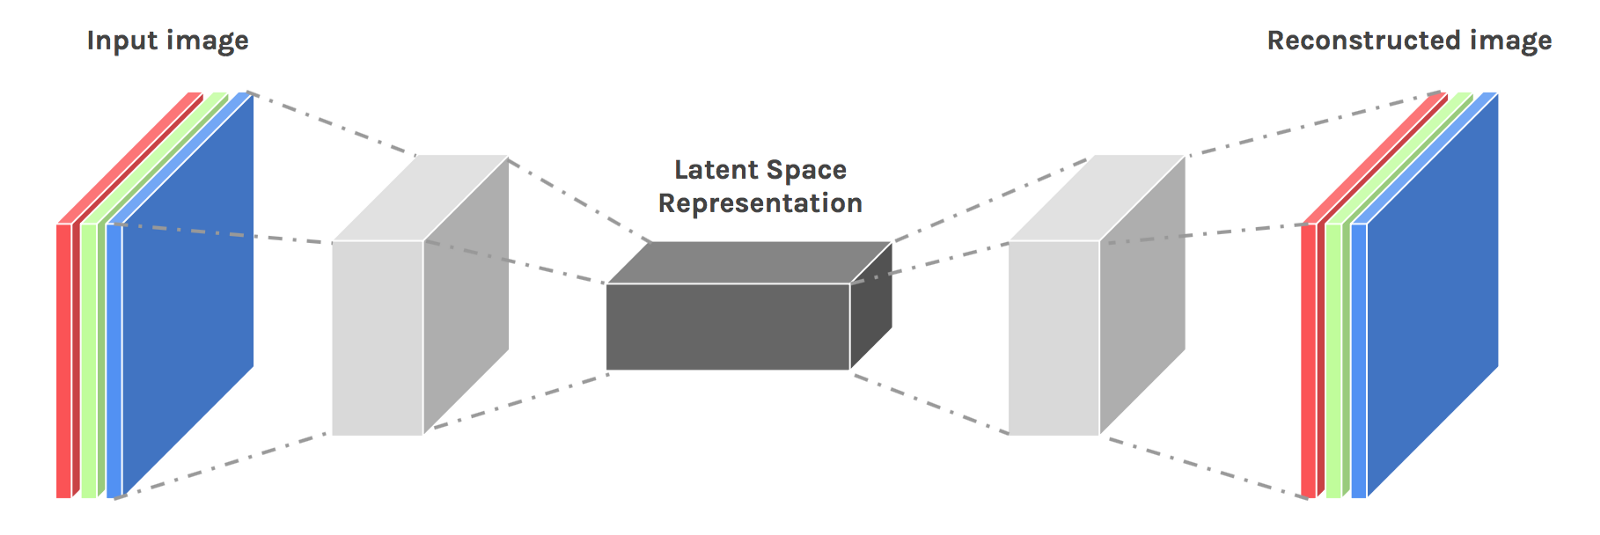
\includegraphics[height=0.9\textheight, width=\textwidth, keepaspectratio]{images/autoencoders/architecture.png}
%     \caption{Autoencoder architecture}
% \end{figure}

% \framebreak

\textbf{Design Considerations}:
\small
\begin{itemize}
    \item \textbf{How deep?} More layers can learn more, but also make training harder and risk overfitting.
    \item \textbf{How wide?} More neurons per layer can help, but too many may just copy the input instead of learning.
    \item \textbf{Symmetry:} Encoder and decoder can look the same, but don’t have to—sometimes different shapes work better.
    \item \textbf{Regularization:} Tricks like dropout or weight penalties help prevent the model from just memorizing.
    \item \textbf{Latent size:} The “bottleneck” size is key—too small loses info, too big doesn’t compress.
    \item \textbf{Activation:} Functions like ReLU or sigmoid help the network learn complex patterns.
\end{itemize}
\normalsize

\framebreak

\textbf{Encoder}:
\begin{itemize}
    \item Takes input data (e.g., image, text, audio)
    \item Uses neural layers to reduce it to a smaller dimension
    \item Learns to keep only the important features
    \item \textit{Example}: 784-pixel image to 32 numbers
\end{itemize}

\framebreak
\textbf{Latent Space (Bottleneck)}:
\begin{itemize}
    \item This is the core representation of the data
    \item It's where the model is forced to be efficient
    \item If too big: model memorizes; too small: model forgets
    \item Sweet spot = good generalization
\end{itemize}

\framebreak

\textbf{Decoder}:
\begin{itemize}
    \item Takes the bottleneck output
    \item Expands it back to the original input size
    \item Tries to make it as close as possible to the real input
    \item Learns to generate data from compressed features
    \item \textit{Example}: Converts 32 numbers back to a 784-pixel image
\end{itemize}

\framebreak

\begin{table}[h!]
\centering
\begin{tabular}{|>{\raggedright\arraybackslash}m{2cm}|>{\raggedright\arraybackslash}m{8cm}|}
\hline
\textbf{Component} & \textbf{Description} \\
\hline
Encoder & Transforms the input data into a compressed latent representation using layers such as Dense, Convolutional, or Recurrent layers. \\
\hline
Latent Space (Bottleneck) & The central compact representation of the input. Forces the model to learn the most essential features. \\
\hline
Decoder & Reconstructs the input from the latent space. Typically mirrors the encoder’s structure in reverse. \\
\hline
Loss Function & Measures the difference between input and output (e.g., Mean Squared Error, Binary Cross-Entropy). Drives learning during training. \\
\hline
Training & Involves minimizing reconstruction error using gradient-based optimization methods such as SGD or Adam. \\
\hline
\end{tabular}
\caption*{Architecture Summary Table}
\end{table}

\framebreak

\begin{figure}
    \centering
    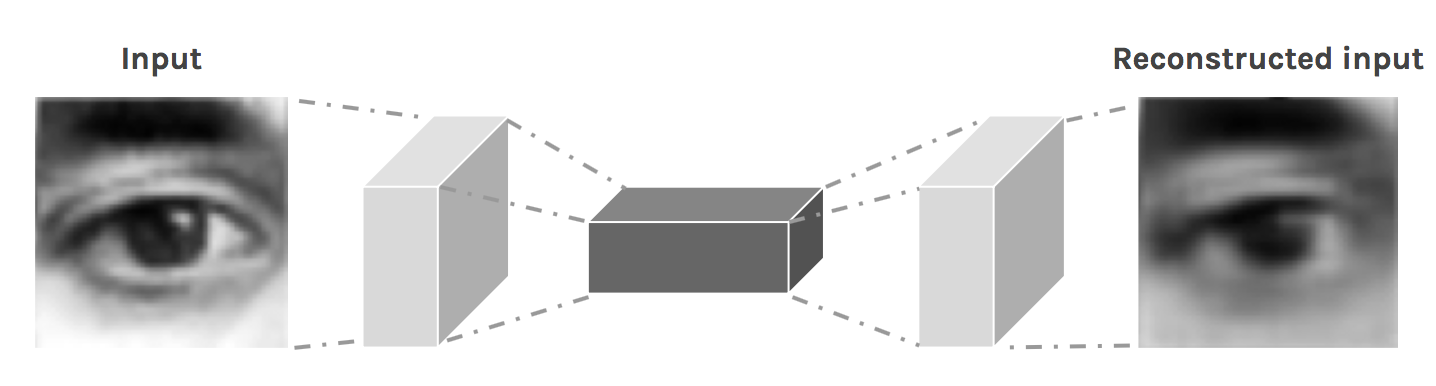
\includegraphics[height=0.9\textheight, width=\textwidth, keepaspectratio]{images/autoencoders/sample.png}
    \caption*{Sample Autoencoder}
\end{figure}
\end{frame}

\begin{frame}{Autoencoders: Interactive Demo}
    \centering
    \href{https://douglasduhaime.com/posts/visualizing-latent-spaces.html}{https://douglasduhaime.com/posts/visualizing-latent-spaces.html}
\end{frame}